% !TeX spellcheck = en_US
\chapter{Policy Gradient}

The Policy Gradient approach has a neural network (\figref{fig:policy-gradient}) to learn and optimize the policy (the blue box in \figref{fig:RL-structure}). This is a model-free \ac{RL} approach. For most model-free \ac{RL} approach, we assume that we don't know the transition model $p(\textbf{s}_{t+1} | \textbf{s}_t, \textbf{a}_t)$ or the initial state \ac{prob} $p(\textbf{s}_1)$. However, we assume that we can interact with the real world to sample the data.

\begin{figure}[hbt!]
	\centering
	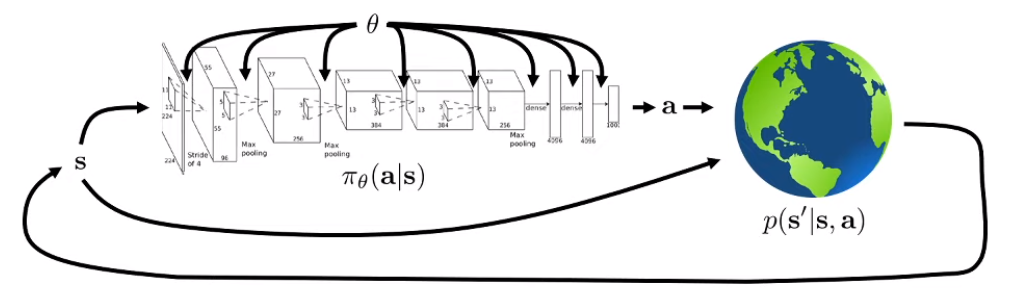
\includegraphics[width=.7\textwidth]{policy-gradient.png}
	\caption{The policy network $\pi_{\theta}(\textbf{a}|\textbf{s})$ with \ac{param} $\theta$. The network takes the current state $\textbf{s}_t$ as input, learn the policy $\pi_{\theta}(\textbf{a}_t|\textbf{s}_t)$ by optimizing \ac{param} $\theta$, and output the action $\textbf{a}_t$.}
	\label{fig:policy-gradient}
\end{figure}

\section{Approach}
\hlb{Goal:} to maximize the expectation of total rewards, which will be denoted as $J(\theta)$
\begin{align}
	\tau & = \{ \textbf{s}_1, \textbf{a}_1, \dots, \textbf{s}_T, \textbf{a}_T \} && \text{denotes the trajectory}\\
	p_\theta(\tau) & = p_\theta(\textbf{s}_1, \textbf{a}_1, \dots, \textbf{s}_T, \textbf{a}_T) && \text{\ac{prob} of the trajectory} \label{eq:traj-prob}\\
	& = p(\textbf{s}_1) \prod_{t=1}^T \pi_{\theta}(\textbf{a}_t | \textbf{s}_t) p(\textbf{s}_{t+1} | \textbf{s}_t, \textbf{a}_t)\\
	\theta^* & = \underset{\theta}{\arg\max} \;\mathbb{E}_{\tau\sim p_\theta(\tau)} \left[ \sum_t r(\textbf{s}_t, \textbf{a}_t) \right] && \text{\ac{RL} goal}\\
	& = \underset{\theta}{\arg\max}\;\mathbb{E}_{(\textbf{s,a})\sim p_\theta(\textbf{s,a})} [r(\textbf{s, a})] && \text{\textbf{infinite} horizon case}\\
	& = \underset{\theta}{\arg\max} \sum_{t=1}^{T} \mathbb{E}_{(\textbf{s}_t,\textbf{a}_t)\sim p_\theta(\textbf{s}_t,\textbf{a}_t)} [r(\textbf{s}_t,\textbf{a}_t)] && \text{\textbf{finite} horizon case}\\
	& = \underset{\theta}{\arg\max} J(\theta)\\
	J(\theta) & = \mathbb{E}_{\tau\sim p_\theta(\tau)} \left[ \sum_{t=1}^T r(\textbf{s}_t, \textbf{a}_t) \right]\\
	& = \mathbb{E}_{\tau\sim p_\theta(\tau)} [r(\tau)] = \int p_\theta(\tau) r(\tau) d\tau
\end{align}

Even though we do not know the initial state \ac{prob} $p(\textbf{s}_1)$ and the transition model $p(\textbf{s}_{t+1} | \textbf{s}_t, \textbf{a}_t)$, we do have the ability to interact with the world and take samples from it. Thus, we can simply take $N$ trajectory samples $\tau_i$ and take the average of them to approximate the expectation of $J(\theta)$. The higher the number of sample trajectories $N$ is, the better the approximation accuracy.
\begin{equation}
	J(\theta) \approx \frac{1}{N} \sum_{i}^N \sum_{t} r(\textbf{s}_{i,t}, \textbf{a}_{i, t}) \qquad \text{sum over samples and time steps}
\end{equation}

\hlb{The Policy Gradient:}
\begin{align}
	\nabla_\theta J(\theta) &= \int \nabla_\theta p_\theta(\tau)r(\tau)d\tau = \int p_\theta(\tau)\nabla_\theta\log p_\theta(\tau)r(\tau)d\tau \label{eq:policy-grad} \\
	&= \mathbb{E}_{\tau\sim p_\theta(\tau)} \left[ \nabla_\theta\log p_\theta(\tau) r(\tau) \right] \label{eq:pg-1}\\
	&= \mathbb{E}_{\tau\sim p_\theta(\tau)} \left[ \left( \sum_{t=1}^{T} \nabla_\theta\log \pi_\theta(\textbf{a}_{t} | \textbf{s}_{t} ) \right) \left( \sum_{t=1}^{T} r(\textbf{s}_{t}, \textbf{a}_{t}) \right) \right] \label{eq:pg-2}
\end{align}
{\color{red} \begin{subequations}
		\begin{empheq}[box=\widefbox]{align}
			\nabla_\theta J(\theta) & \approx \frac{1}{N} \sum_{i=1}^{N} \left[ \left( \sum_{t=1}^{T} \nabla_\theta\log \pi_\theta(\textbf{a}_{i,t} | \textbf{s}_{i,t} ) \right) \left( \sum_{t=1}^{T} r(\textbf{s}_{i,t}, \textbf{a}_{i,t}) \right) \right]\\
			\text{\underline{then}} \quad \theta &\leftarrow \theta + \alpha \nabla_\theta J(\theta)
		\end{empheq}
\end{subequations}}

\hlr{\underline{REMARKS}:}
\begin{itemize}
	\item some what like \ac{MLE}, makes good stuff happen more, bad stuff happens less
	\item Transition in \eqref{eq:policy-grad} happens due to a convenient identity transformation:
	\begin{equation*}
		p_\theta(\tau) \nabla_\theta \log p_\theta(\tau) = p_\theta(\tau) \frac{\nabla_\theta p_\theta(\tau)}{p_\theta(\tau)} = \nabla_\theta p_\theta(\tau)
	\end{equation*}
	\item Taking the $\log$ of $p_\theta(\tau)$ in \eqref{eq:traj-prob} then replacing it into \eqref{eq:pg-1} leads to \eqref{eq:pg-2}
\end{itemize}

\section{Partial Observability}
\begin{align*}
	\nabla_\theta J(\theta) & \approx \frac{1}{N} \sum_{i=1}^{N} \left[ \left( \sum_{t=1}^{T} \nabla_\theta\log \pi_\theta(\textbf{a}_{i,t} | o_{i,t}) \right) \left( \sum_{t=1}^{T} r(\textbf{s}_{i,t}, \textbf{a}_{i,t}) \right) \right]\\
	& \qquad o_{i, t} \rightarrow \underset{\pi_\theta(\textbf{a}_{i,t} | o_{i,t})}{\text{network}} \rightarrow \textbf{a}_{i,t}
\end{align*}
Markov property is not actually used! $\Rightarrow$ can use policy gradient for \ac{POMDP}s without modification

\section{High Variance Problem}
In general, when we add a constant (either positive or negative) to the rewards, the policy should be the same. However, this is not the case for the above derivation of policy gradient. The change of policy distribution varies depends on the value of the total rewards $r(\tau)$. In other words, the problem is \hlr{\underline{HIGH VARIANCE} with $r(\tau)$}.
\begin{itemize}
	\item Different samples $\Rightarrow$ different gradient estimate
	\item For a small finite \ac{no} samples $\Rightarrow$ noisy gradient\\
	(At the beginning, policy $\theta$ is not so good $\Rightarrow$ random action $\Rightarrow$ the not-so-good action results accumulate $\Rightarrow$ high variance in the end)
\end{itemize}

\hlb{Solution:} reducing variance
\begin{itemize}
	\item \textit{Causality:} policy at time $t'$ cannot affect reward at time $t$, when $t'<t$
	\begin{align}
		\Rightarrow\; \nabla_\theta J(\theta) & \approx \frac{1}{N} \sum_{i=1}^{N} \left[ \left( \sum_{t=1}^{T} \nabla_\theta\log \pi_\theta(\textbf{a}_{i,t} | \textbf{s}_{i,t} ) \right) \left( \sum_{\color{red} t'=t}^{T} r(\textbf{s}_{i,t'}, \textbf{a}_{i,t'}) \right) \right]\\
		& \approx \frac{1}{N} \sum_{i=1}^{N} \sum_{t=1}^{T} \nabla_\theta\log \pi_\theta(\textbf{a}_{i,t} | \textbf{s}_{i,t} ) \widehat{Q}_{i,t} \qquad\quad (\widehat{Q}_{i,t} \text{ - the reward to-go})
		\label{eq:Q-value}
	\end{align}
	This leads to smaller variance, because $\widehat{Q}_{i,t}$ is smaller than the total rewards, and the expectation of smaller number has smaller variance.
	\item \textit{Baselines:} the average of total rewards over different trajectories
	\begin{align}
		b &= \frac{1}{N} \sum_{i=1}^{N}r(\tau)\\
		\nabla_\theta J(\theta) & \approx \frac{1}{N} \sum_{i=1}^{N} \nabla_\theta\log \pi_\theta(\tau) [r(\tau)-b]\\
		& {\color{red} r(\tau)-b = Q^\pi(\textbf{s}_t, \textbf{a}_t) - V^\pi(\textbf{s}_t)}
	\end{align}
	It is proven that subtracting the baseline is unbiased in expectation. This is not the best baseline to reduce the variance, but it's simple and good enough.
\end{itemize}

\section{Off-policy Policy Gradient}
Vanilla Policy Gradient is on-policy, since we have $\tau\sim\ p_\theta(\tau)$. This poses a problem, since the neural networks change only a bit with each gradient step. Off-policy Policy Gradient can be derived with \hlr{Important sampling}:
\begin{align}
	\mathbb{E}_{x\sim p(x)}[f(x)] &= \mathbb{E}_{x\sim q(x)} \left[\frac{p(x)}{q(x)}f(x)\right]\\
	\Rightarrow \quad \nabla_{\theta'} J(\theta') & = \mathbb{E}_{\tau \sim p_{\theta}(\tau)} \left[ \frac{\nabla_{\theta'} p_{\theta'}(\tau)}{p_{\theta}(\tau)} r(\tau) \right]\\
	&= \mathbb{E}_{\tau \sim p_{\theta}(\tau)} \left[ \frac{p_{\theta'}(\tau)}{p_{\theta}(\tau)} \nabla_{\theta'}\log p_{\theta'}(\tau) r(\tau) \right]\\
	&\approx \frac{1}{N} \sum_{i=1}^N \sum_{t=1}^T \frac{\pi_{\theta'}(\textbf{a}_{i,t} | \textbf{s}_{i,t})}{\pi_{\theta}(\textbf{a}_{i,t} | \textbf{s}_{i,t})} \nabla_{\theta'} \log \pi_{\theta'} (\textbf{a}_{i,t} | \textbf{s}_{i,t}) \widehat{Q}_{i,t}
\end{align}
with $\theta'$ as the \textit{new} \ac{param} and $\theta$ as the \textit{old} \ac{param}

\section{REINFORCE Algorithm}
\begin{enumerate}
	\item \tikzmark{pg1}Sample $\{\tau_i\}$ from $\pi_\theta(\textbf{a}_t|\textbf{s}_t)$ policy
	\item $\displaystyle \nabla_\theta J(\theta) \approx \frac{1}{N} \sum_{i=1}^{N} \nabla_\theta\log \pi_\theta(\tau) \left(\sum_{t'=t}^{T} r(\textbf{s}_{i,t'}, \textbf{a}_{i, t'})\right)$\\
	\item \tikzmark{pg3}$\theta \leftarrow \theta + \alpha \nabla_\theta J(\theta)$ \qquad\qquad \cite{williams1992jml}
	\begin{tikzpicture}[overlay,remember picture]
		\draw[very thick, -latex] ([xshift=-7mm,yshift=1mm]pic cs:pg3) --++ (-.5,0) |- ([xshift=-7mm,yshift=1mm]pic cs:pg1);
	\end{tikzpicture}
\end{enumerate}

\hlr{Pseudo code:} (\texttt{tensorflow})\\
When coding, use the pseudo loss as a weighted maximum likelihood:
\begin{equation}
	\widetilde{J}(\theta) \approx \frac{1}{N} \sum_{i=1}^{N} \sum_{t=1}^{T} \log \pi_{\theta} (\textbf{a}_{i,t} | \textbf{s}_{i,t} ) \widehat{Q}_{i,t}
\end{equation}
\texttt{logits = policy.predictions(states)}\\
\texttt{negative\_likelihoods = tf.nn.softmax\_cross\_entropy(labels = actions, logits)}\\
\texttt{weighted\_negative\_likelihoods = tf.multiply(negative\_likelihoods, q\_values)}\\
\texttt{loss = tf.reduce\_mean(weighted\_negative\_likelihoods)}\\
\texttt{gradients = loss.gradients(loss, variables)}

with \texttt{q\_values} already taking causality and baselines into account.

\section{Natural Policy Gradient}

Natural Policy gradients, \ac{aka}, covariant policy gradient, apply a trick to change the learning rate for different parameters. The high-level idea is such that some \ac{param} change \ac{prob} a lot more than others. In other words, the vanilla policy gradient apply a constraint on the \ac{param} space rather than the policy space. But with every gradient step, we rather want a constant step in the policy space. \cite{peters2008nn}

\begin{align}
	&\theta' \leftarrow \underset{\theta'}{\arg\max} (\theta'-\theta)^T \nabla_\theta J(\theta) \quad \text{\ac{st} } ||\theta' - \theta||^2 \leq \epsilon \quad \text{(\ac{param} space)}\\
	&\theta' \leftarrow \underset{\theta'}{\arg\max} (\theta'-\theta)^T \nabla_\theta J(\theta) \quad \text{\ac{st} } D(\pi_{\theta'}, \pi_{\theta}) \leq \epsilon \quad \text{(policy space)}
\end{align}

A good choice for $D(\pi_{\theta'}, \pi_{\theta})$ is the \ac{KL}-divergence. To simplify the process, the \ac{KL}-divergence is approximated with Fisher information matrix:q

\begin{align}
	& D_{KL}(\pi_{\theta'} || \pi_{\theta}) \approx (\theta' - \theta)^T \textbf{F} (\theta' - \theta)\\
	& \textbf{F} = \mathbb{E}_{\pi_{\theta}} [ \nabla_\theta \log\pi_\theta(\textbf{a}|\textbf{s}) \nabla_\theta \log \pi_\theta (\textbf{a}|\textbf{s})^T ] && \text{Fisher information matrix}\\
	& \theta' \leftarrow \underset{\theta'}{\arg\max} (\theta'-\theta)^T \nabla_\theta J(\theta) \quad \text{\ac{st} } ||\theta' - \theta||^2_\textbf{F} \leq \epsilon\\
	& \theta \leftarrow \theta + \alpha \textbf{F}^{-1} \nabla_\theta J(\theta)
\end{align}

\section{References}
\begin{itemize}
	\item \citeaus{peters2008nn}. Reinforcement learning of motor skills with policy gradients.
	\item \citeaus{levine2013icml}. Guided policy search: deep \ac{RL} with importance sampled policy gradient.
	\item \citeausm{schulman2015icml}. Trust region policy optimization: deep \ac{RL} with natural policy gradient and adaptive step size.
	\item \citeausm{schulman2017proximal}. Proximal policy optimization algorithms: deep \ac{RL} with importance sampled policy gradient
\end{itemize}